\section{Outlook}


\subsection{}
\begin{frame}
\frametitle{Outlook}
	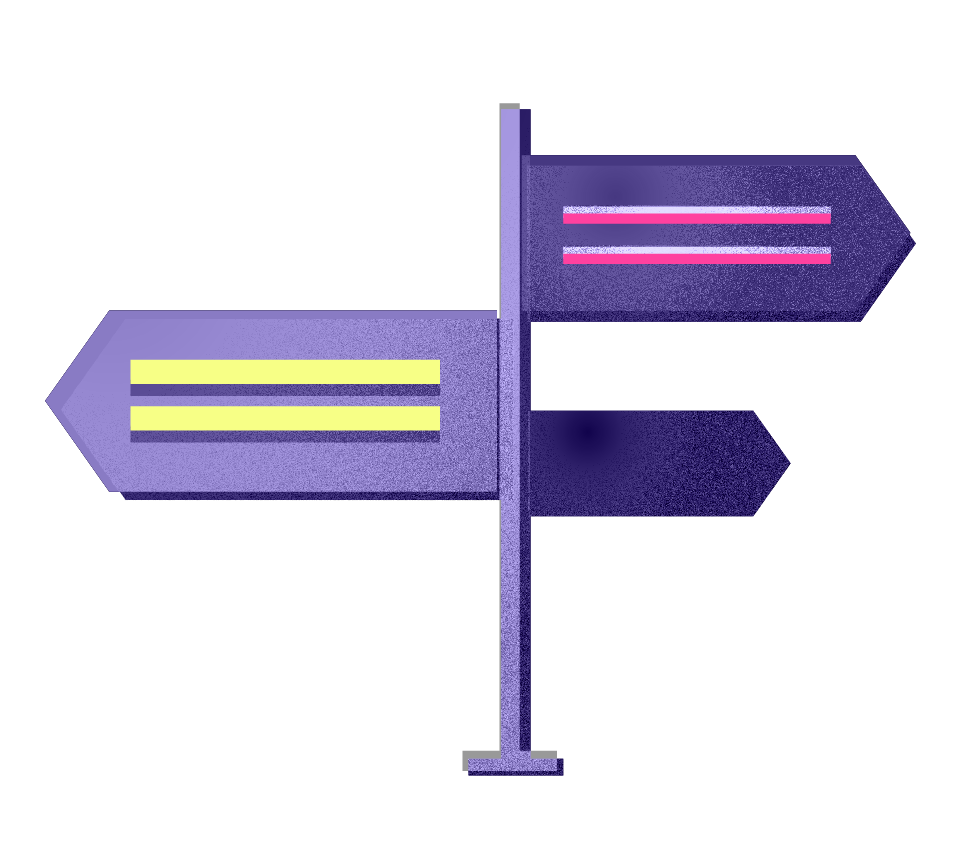
\includegraphics[width=0.9\textwidth]{img/plan.png}
\end{frame}

\subsection{Exception handling}
\begin{frame}
\frametitle{Exception handling}
\begin{itemize}
	\item Exceptions are good
	\begin{itemize}
		\item Exceptions help to fix problems
		\item Exceptions help in case of data corruption	
	\end{itemize}
	\item More exceptions
	\item E.g. instead of return values
\end{itemize}
\end{frame}

\subsection{Easier initialization}
\begin{frame}
\frametitle{Easier initialization}
\begin{itemize}
	\item A lot of boilerplate code is required to get started with a standalone application
	\item Goal: reduce that
\end{itemize}
\end{frame}

\subsection{More pythonic constructs}
\begin{frame}
\frametitle{More pythonic constructs}
\begin{itemize}
	\item More decorators
	\item More iterators
\end{itemize}
\end{frame}

\subsection{Nice API}
\begin{frame}
\frametitle{Nice API}
\begin{itemize}
	\item But that is not Python specific
\end{itemize}
\end{frame}

\subsection{Start Coding}
\begin{frame}
\frametitle{Start Coding}
	\begin{columns}[T] % contents are top vertically aligned
		\begin{column}[T]{5cm} % each column can also be its own environment
		\begin{itemize}
			\item Let's get to work
		\end{itemize}
		\end{column}
		\begin{column}[T]{5cm} % alternative top-align that's better for graphics
			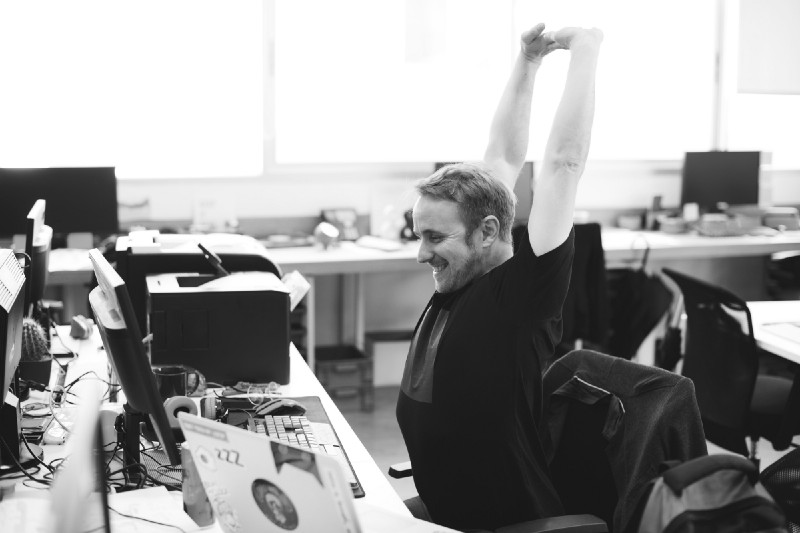
\includegraphics[height=3.5cm]{img/start_coding.jpg}
		\end{column}
	\end{columns}
\end{frame}

\subsection{Thank you}
\begin{frame}
\frametitle{Thank you}
Questions?
Now or later...
\end{frame}
